% Formula sheet for MEC E 331 Fluid mechanics 1
% Two column format

\documentclass[10pt]{article}
\usepackage{amsmath}
\usepackage{amssymb}
\usepackage{multicol}
\usepackage{geometry}
\usepackage{fancyhdr}
\usepackage{siunitx}
\usepackage{enumitem}
\usepackage{multicol}
\usepackage{graphicx}
\usepackage{multirow}
\usepackage{lastpage}
\usepackage[final]{hyperref}
\usepackage{parskip}
\usepackage{nccmath}
\usepackage{float}

\DeclareRobustCommand{\volume}{\text{\volumedash}V}
\newcommand{\volumedash}{%
  \makebox[0pt][l]{%
    \ooalign{\hfil\hphantom{$\m@th V$}\hfil\cr\kern0.08em--\hfil\cr}%
  }%
}

\geometry{letterpaper, portrait, margin=0.5in, footskip=0.25in, top = 0.75in, headsep=0.25in}
%\setlength{\columnsep}{0.5in}

\hypersetup{
	colorlinks=true,       % false: boxed links; true: colored links
	linkcolor=blue,        % color of internal links
	citecolor=blue,        % color of links to bibliography
	filecolor=magenta,     % color of file links
	urlcolor=blue         
}

\pagestyle{fancy}
\fancyhf{}
\lhead{MEC E 331 Formula Sheet}
\chead{Last Updated: \today}
\rhead{Alex Diep}
\cfoot{\thepage\ of \pageref{LastPage}}
%add line for footer 
% \renewcommand{\footrulewidth}{0.4pt}% default is 0pt


% set head height and top = 1.2cm
\setlength{\headheight}{15pt}

\begin{document}
%\maketitle
%\thispagestyle{empty}
\begin{multicols*}{2}
\section*{5. \& 8. Bernoulli-Energy Methods}
\subsection*{5.1 General Procedure}
\begin{enumerate}
    \item There are 2 equations that are generally useful for these types of problems:
    \begin{enumerate}[label=\roman*)]
        \item Bernoulli's equation. Valid in regions of steady, incompressible 
        flow where net frictional forces are negligible.
        \item Mass flow rate: $\dot{m} = \rho A \dot{x} = \rho V$
    \end{enumerate}
    \item Identify the assumptions so the appropriate equations can be used.
    \item Try and cancel out as many terms as possible from the Bernoulli equation. Use mass flow rate to determine $\dot{x}$.
    \item Use energy methods to determine the pressure head if necessary.
\end{enumerate}
\subsection*{5.2 Variable Definitions}
\begin{itemize}
    \item $P$: Pressure
    \item $\dot{x}$: Velocity
    \item $z$: Elevation
    \item $V$: Volume
    \item $C_d$: Discharge coefficient
    \item $\beta$: Ratio of throat diameter to pipe diameter $d/D$
\end{itemize}
\subsection*{5.3 Formulas}
Classic Bernoulli Equations:
\begin{fleqn}
    \begin{align*}
        &\text{Bernoulli's Equation: } \frac{P_1}{\rho} + \frac{\dot{x}_1^2}{2} + gz_1 = \frac{P_2}{\rho} + \frac{\dot{x}_2^2}{2} + gz_2 \\
        &\text{Mass Conservation: } \Delta m_{\text{CV}} = \dot{m}_{\text{in}} - \dot{m}_{\text{out}} \\
        &\text{Mass Flow Rate: } \dot{m} = \rho A \dot{x} = \rho V \\
    \end{align*}
\end{fleqn}
Obstruction flowmeter:
\begin{figure}[H]
    \centering
    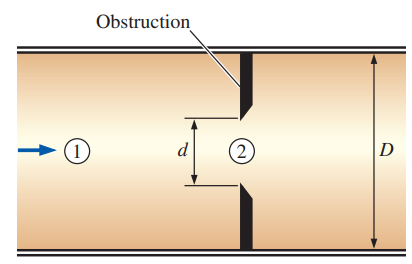
\includegraphics[width=0.2\textwidth]{Figures/Sec8 Obstruction Flowmeter.png}
    \caption{Obstruction flowmeter}
    \label{fig:obstruction_flowmeter}
\end{figure}
\begin{fleqn}
    \begin{align*}
        &\text{Obstruction flowmeter: } \dot{V} = A_0 C_d \sqrt{\frac{2(P_1 - P_2)}{\rho (1 - \beta^4)}} \\
        &\text{Mass Balance : } \implies \dot{x}_1 = (d/D)^2 \dot{x}_2 \\
        &\text{Head Loss: } h_L = \frac{P_1}{\rho g} + \frac{\dot{x}_1^2}{2g} + z_1 - \frac{P_2}{\rho g} - \frac{\dot{x}_2^2}{2g} - z_2 \\
    \end{align*}
\end{fleqn}
\section*{6. Momentum Analysis of Flow Systems}
\subsection*{6.1 General Procedure}
\begin{enumerate}
    \item Utilize the Bernoulli equation to obtain the $P_{1, \text{gage}}$
    \item $\sum \vec{F}$ represents external forces acting on the system. Some examples are:
    \begin{enumerate}[label=\roman*)]
        \item Pressure: $P_{1, \text{gage}} A_1$
        \item Reaction force: $F_{R}$
    \end{enumerate}
    \item Use momentum equation to obtain forces. For uniform flow, $\beta = 1$.  If not given, 
    it is expected to assume uniform flow.
\end{enumerate}

\subsection*{6.2 Variable Definitions}
\begin{itemize}
    \item $\beta$: Momentum-flux correction factor. It's a correction factor for the surface integral.
\end{itemize}

\subsection*{6.3 Formulas}
\begin{fleqn}
    \begin{align*}
        &\text{Momentum Equation: } \sum \vec{F} = \sum_{\text{out}} \beta \dot{m} \vec{V} - \sum_{\text{in}} \beta \dot{m} \vec{V} \\
        &\text{Momentum Correction Factor: } \beta = \begin{cases}
            4/3 & \text{laminar} \\
            1 & \text{turbulent}
        \end{cases} \\ 
    \end{align*}
\end{fleqn}
\section*{9. Differential Analysis of Fluid Flow}
\subsection*{9.1 General Procedure}
\begin{enumerate}
    \item Most problems will be simplifiable to 2D or 1D because full form Navier-Stokes equations are too difficult to solve. The art of these 
    problems is to simplify the equations to a form that can be solved.
    \item Common assumptions are: steady, laminar, incompressible, constant viscosity, constant pressure, constant temperature, and
    parallel flow (velocity only in one direction). Gravity typically acts in the negative z-direction (unless it's like an inclined 
    plane where you'd set your coordinates to be tangential and normal to the plane).
    \item Check the problem statement for these key words: %steady, laminar, incompressible, constant density, constant viscosity, constant pressure,\
    \begin{enumerate}[label=\roman*)]
        \item Steady: All $\frac{\partial}{\partial t} = 0$
        \item Laminar: Generally implies parallel flow, flow in one direction only.
        \item Incompressible: $\text{div}(\vec{V}) = \nabla \cdot \vec{V} = 0$, $\frac{\partial \rho}{\partial t} = 0$
        \item Pressure acts in only one-direction: $\frac{\partial P}{\partial x} = 0$, $\frac{\partial P}{\partial y} = 0$, or $\frac{\partial P}{\partial z} = 0$ 
        \item Parallel flow: Velocity in the direction of motion is non-zero, velocity in the other directions is zero.
        \item Gravity only in z-direction: $\vec{g} = -g \hat{k}$
    \end{enumerate}
    \item Boundary conditions:
    \begin{enumerate}[label=\roman*)]
        \item No-slip: $\vec{V}_{\text{fluid}} = \vec{V}_{\text{boundary}}$ at an interface boundary.
        \item No-shear at a : $\tau_{\text{fluid}} = \tau_{\text{boundary}} \approx 0$ at a free surface boundary with small surface tension like air.
    \end{enumerate}
    \item Try to simplify the continuity equation first. Use the results in simplifying the Navier-Stokes equation.
    \item Solve for whatever is asked for in the problem statement.
\end{enumerate}

\subsection*{9.2. Operator Definitions}
\begin{itemize}
    \item $\nabla$: The gradient operator, $\nabla = \frac{\partial}{\partial x} \hat{i} + \frac{\partial}{\partial y} \hat{j} + \frac{\partial}{\partial z} \hat{k}$
    \item $\frac{\partial \vec{V}}{\partial x}$: The vector partial derivative, 
    $\frac{\partial \vec{V}}{\partial x} = \frac{\partial u}{\partial x} \hat{i} + \frac{\partial v}{\partial x} \hat{j} + \frac{\partial w}{\partial x} \hat{k}$
    \item $\frac{D}{Dt}$: The material derivative, $\frac{D \vec{T}}{Dt} = \frac{\partial \vec{T}}{\partial t} + (\vec{V} \cdot \nabla) \vec{T}$
    \footnote[1]{$(\vec{V} \cdot \nabla)$ is the convective derivative operator, not div($\vec{V}$)}
    \item $(\vec{V} \cdot \nabla)$: The convective derivative, $(\vec{V} \cdot \nabla) \vec{T} = u \frac{\partial \vec{T}}{\partial x} + v \frac{\partial \vec{T}}{\partial y} + w \frac{\partial \vec{T}}{\partial z}$
    \item $\nabla^2$: The Laplacian operator, $\nabla^2 = \frac{\partial^2}{\partial x^2} + \frac{\partial^2}{\partial y^2} + \frac{\partial^2}{\partial z^2}$
\end{itemize}

\subsection*{9.3 Variable Definitions}
\begin{itemize}
    \item $\vec{V}$: Velocity vector, $\vec{V} = u \hat{i} + v \hat{j} + w \hat{k}$
    \item $\rho$: Density
    \item $\mu$: Viscosity
    \item $P$: Pressure
\end{itemize}

\subsection*{9.4 Formulas}
\begin{fleqn}
\begin{align*}
    &\text{Continuity Equation: } \frac{\partial \rho}{\partial t} + \nabla \cdot (\rho \vec{V}) = 0 \\
    % &\text{Cartesian: } \frac{\partial \rho}{\partial t} + \frac{\partial}{\partial x}(\rho u) + \frac{\partial}{\partial y}(\rho v) 
    % + \frac{\partial}{\partial z}(\rho w) = 0 \\
    % &\text{Cylindrical: } \frac{\partial \rho}{\partial t} + \frac{1}{r} \frac{\partial(r \rho u)}{\partial r} + \frac{\partial(\rho v)}{\partial \theta} 
    % + \frac{\partial(\rho w)}{\partial z} = 0 \\
    &\text{Special Case 1: Steady Compressible Flow: } \nabla \cdot (\rho \vec{V}) = 0 \\
    &\text{Special Case 2: Incompressible Flow: } \nabla \cdot \vec{V} = 0 \\
    &\text{Incompressible flow, Newtonian, Navier-Stokes Equation:}
\end{align*}
\end{fleqn}
\begin{align*}
    \rho \frac{ D \vec{V}}{D t}  &= -\nabla P + \rho \vec{g} + \mu \nabla^2 \vec{V} 
\end{align*}
For example in x-direction:
\begin{align*}
    \rho \left(\frac{\partial u}{\partial t} + u \frac{\partial u}{\partial x} + v \frac{\partial u}{\partial y} + w \frac{\partial u}{\partial z}\right) 
    = &-\frac{\partial P}{\partial x} + \rho g_x \\
    &+ \mu \left(\frac{\partial^2 u}{\partial x^2} + \frac{\partial^2 u}{\partial y^2} + \frac{\partial^2 u}{\partial z^2}\right)
\end{align*}
\subsection*{9.5 General Terms}
\begin{itemize}
    \item Control volume analysis: very useful tool to engineering for flow analysis. Gives 'engineering analysis' answer, sometimes crude approximation, but always useful.
    A method of analysis in which a volume in space is selected and the conservation of mass, momentum, and energy are applied to the volume
    \item Differential analysis:  in principle can be used for any problems. In practice, limited cases where exact analytical solutions exist. 
    Nowadays, CFD (computational fluid dynamics) simulations are widely performed based on differential analysis. Involves application of differential 
    equations of fluid motion to any and every point in the flow field over a region called the flow domain.
    Experimental (dimensional) analysis: based on the results of experiments. Technique to derive the most use out of the fewest number of experiments 
    (which cost time and money)
\end{itemize}
\section*{10. Boundary Layer Approximation}
\subsection*{10.1 General Procedure}
\begin{enumerate}
    \item Identify the type of flow using the Reynolds number. If the Re $> 5 \times 10^5$, the flow is turbulent. If the Re $< 5 \times 10^5$, the flow is laminar.
    \item Use Table \ref{tab:boundary_layer_approximation} to determine whatever you need.
\end{enumerate}

\subsection*{10.2 Variable Definitions}

\subsection*{10.3 Formulas}
\begin{fleqn}
    \begin{align*}
        &\text{Reynolds Number: } \text{Re}_x = \frac{\rho V x}{\mu}  = \frac{V x}{\nu} \\
        &\text{Boundary Layer Thickness: } \frac{\delta}{x} = 4.91 \sqrt{\text{Re}_x} \\
        &\text{Wall Shear Stress: } \tau_w = \frac{0.332 \rho U^2}{\sqrt{\text{Re}_x}} \\
        &\text{Local Friction Coefficient: } C_f = \frac{\tau_w}{\frac{1}{2} \rho U^2} = \frac{0.664}{\sqrt{\text{Re}_x}} \\
        &\text{Displacement Thickness: } \delta^* = \int_0^\infty \left(1 - \frac{u}{U}\right) dy = \frac{1.72 x}{\sqrt{\text{Re}_x}} \\
        &\text{Momentum Thickness: } \theta = \int_0^\infty \frac{u}{U} \left(1 - \frac{u}{U}\right) dy = \frac{0.664 x}{\sqrt{\text{Re}_x}} \\   
        &\text{Drag Force: } F_D = \int_A \tau_w dA = \int_0^L \tau_w w dx \\
        &\text{Continuity Equation: } \frac{\partial u}{\partial x} + \frac{\partial v}{\partial y} = 0 \\
        &\text{Momentum Equation: } u \frac{\partial u}{\partial x} + v \frac{\partial u}{\partial y} = U \frac{dU}{dx} + \nu \frac{\partial^2 u}{\partial y^2} \\
    \end{align*}
\end{fleqn}

\begin{table}[H]
    \caption{Boundary Layer Approximation}
    \label{tab:boundary_layer_approximation}
    \centering
    \begin{tabular}{ccc}
        \hline
        Property & Laminar & Turbulent \\
        \hline
        Boundary Layer Thickness & $\frac{\delta}{x} = 4.91 \sqrt{\text{Re}_x}$ & $\frac{\delta}{x} = \frac{0.16}{(\text{Re}_x)^{1/7}}$ \\
        Displacement Thickness & $\frac{\delta^*}{x} = \frac{1.72}{\sqrt{\text{Re}_x}}$ & $\frac{\delta^*}{x} = \frac{0.020}{(\text{Re}_x)^{1/7}}$ \\
        Momentum Thickness & $\frac{\theta}{x} = \frac{0.664}{\sqrt{\text{Re}_x}}$ & $\frac{\theta}{x} = \frac{0.016}{(\text{Re}_x)^{1/7}}$ \\   
        Local Friction Coefficient & $C_f = \frac{0.664}{\sqrt{\text{Re}_x}}$ & $C_f = \frac{0.027}{(\text{Re}_x)^{1/7}}$ \\
        Wall Shear Stress & $\tau_w = \frac{0.332 \rho U^2}{\sqrt{\text{Re}_x}}$ & $\tau_w = \frac{0.013 \rho U^2}{(\text{Re}_x)^{1/7}}$ \\
        \hline
    \end{tabular}
\end{table}
\end{multicols*}
\end{document}
